% Asset ID: A22FurtherKinematicsTikZ-002
% Unit: A22
% Topic: Further Kinematics
% Related section: Vector SUVAT
\documentclass[tikz,border=8pt]{standalone}
\usepackage{amsmath}
\usetikzlibrary{arrows.meta,positioning,angles,quotes}
\begin{document}

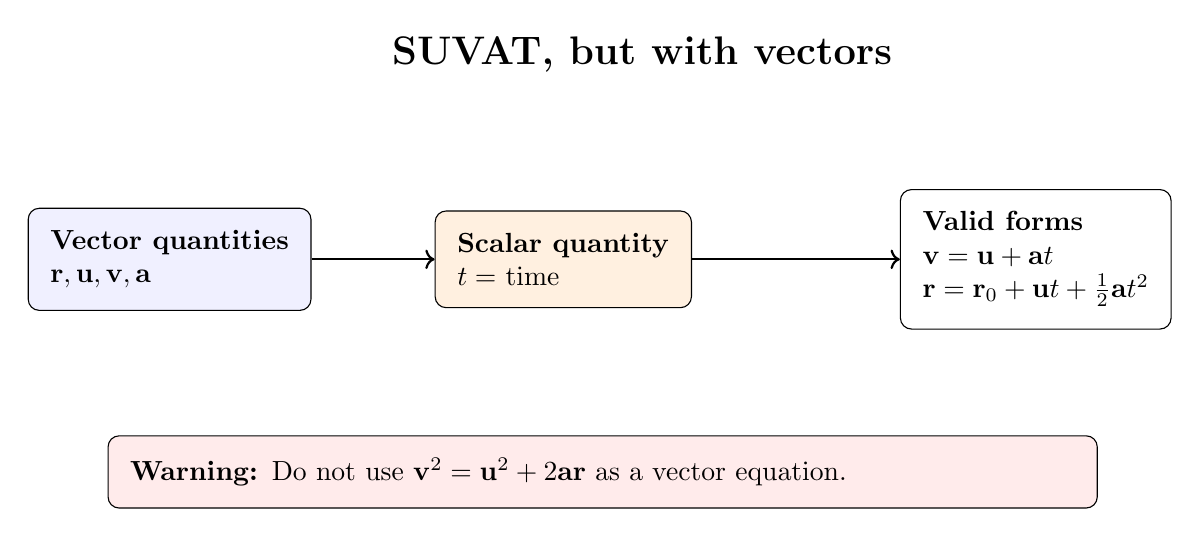
\begin{tikzpicture}[box/.style={draw, rounded corners, fill=white, align=left, inner sep=8pt}, arrow/.style={->, thick}]
\node[font=\bfseries\Large] at (6,6) {SUVAT, but with vectors};
\node[box, fill=blue!6] (v) at (0,3.4) {\textbf{Vector quantities}\\$\mathbf r,\mathbf u,\mathbf v,\mathbf a$};
\node[box, fill=orange!12] (t) at (5,3.4) {\textbf{Scalar quantity}\\$t=$ time};
\node[box] (eq) at (11,3.4) {\textbf{Valid forms}\\$\mathbf v=\mathbf u+\mathbf at$\\$\mathbf r=\mathbf r_0+\mathbf ut+\frac12\mathbf at^2$};
\draw[arrow] (v)--(t); \draw[arrow] (t)--(eq);
\node[box, fill=red!8, text width=12cm] at (5.5,0.7) {\textbf{Warning:} Do not use $\mathbf v^2=\mathbf u^2+2\mathbf a\mathbf r$ as a vector equation.};
\end{tikzpicture}
\end{document}
